% DRAFT for CoRL-style format (8 pages + appendix). Swap in the venue's style file when submitting.
\documentclass[11pt]{article}
\usepackage[margin=1in]{geometry}
\usepackage{amsmath,amssymb,graphicx,booktabs,hyperref}
\newcommand{\E}{\mathbb{E}}
\title{What is a biased simulator worth for evaluating a robot policy?\\ Variance reduction yes, certificates no}
\author{Programme \texttt{sim2real-inference} (written with AI assistance, Claude Code; draft, not submitted)}
\date{}
\begin{document}
\maketitle
\begin{abstract}
A digital twin gives unlimited but biased runs; real trials are unbiased but scarce. We ask how many real trials a twin saves when evaluating a policy, and whether any saving survives a guarantee that holds whatever the twin's bias. On 21 MuJoCo twin--real model pairs (paired correlation $\rho$ from 0.17 to 0.88) a control-variate estimator that pairs twin and real runs on the same context multiplies the effective real sample by up to 3.2, within 6\% of $1/(1-\rho^2)$ at $n=30$ real and $N=300$ twin runs, while unpaired twin runs give none. Plug-in 95\% intervals undercover on the bounded, skewed outcome (down to 86.7\%). Every distribution-free certificate we built (empirical Bernstein, hedged-capital betting, a pilot-checked discrepancy bound, a failure-rate bound, anytime confidence sequences) was valid but never tighter, and up to 3.4 times wider, than its real-only baseline at $n\le 240$. We prove why this is not only a flaw of our constructions: any valid 95\% lower bound has worst-case gap at least $1-(2\delta)^{1/m}\approx 2.3/m$ even for a perfect twin. On real data (SIMPLER's published paired tables, 36 policy--task cells) a leave-one-cell-out calibrated twin has RMSE 0.118 and is worth about 10 real trials (interval 5 to 26). The twin's value is variance reduction for point estimates, not shorter certificates.
\end{abstract}

\section{Introduction}
Real-robot evaluation is the bottleneck of robot learning; generalist policies are often compared on a few dozen real trials with no interval \cite{kressgazit2024empirical}. Simulated evaluation scales but is biased \cite{li2024simpler}. Prediction-powered inference \cite{angelopoulos2023ppi,angelopoulos2023ppipp} gives valid intervals from a small labelled set plus many model predictions, and the classical control variate is its tuned form \cite{peherstorfer2018survey}. A simulator differs from a generic predictor in one way that matters here: it can replay the same scene (context) as the real trial, so twin and real outcomes are paired. We study what that pairing buys and where it stops.
\paragraph{Contributions.} (1) An estimator library and a 21-pair MuJoCo benchmark showing the pairing gain follows $1/(1-\rho^2)$ and unpaired runs give none. (2) A negative result across five certificate constructions. (3) A distribution-free floor, with proof, on any twin-assisted lower bound, tight within about $1.3\times$ at $\delta=0.05$. (4) Two uses of the twin beyond point estimates, active selection of real contexts (gain only where twin error is predictable) and anytime sequences (no gain). (5) A real-data check on SIMPLER's published tables. All claims are pre-registered in the repository's \texttt{LOG.md}, with refuted hypotheses reported.

\section{Setting and estimators}
A context $c$ (initial state, payload, reference) yields a real outcome $R(c)\in[0,1]$ and a twin outcome $T(c)\in[0,1]$. We observe $n$ pairs $(R_i,T_i)$ and $N-n$ extra twin runs, and estimate $\mu=\E R$. The family $\hat\mu_\lambda=\bar R-\lambda(\bar T_{\mathrm{paired}}-\bar T_{\mathrm{all}})$ contains real-only ($\lambda=0$), PPI ($\lambda=1$) and the control variate with $\lambda$ fitted by least squares. It is unbiased for any twin bias. With paired correlation $\rho$ the variance ratio is $E\approx 1/(1-\rho^2(1-n/N))$.

\section{Benchmark}
A torque-driven MuJoCo pendulum arm tracks a sinusoid (a second, unstable task is in the replication paragraph below). The twin is the nominal model; the ``real'' model adds an Ornstein--Uhlenbeck disturbance and one omitted effect (friction, delay, sensor noise, actuator gain, payload mass) at four swept magnitudes, plus a no-effect pair: 21 pairs, 4{,}000 contexts each. These are model-versus-model pairs with swept, not sourced, magnitudes. The disturbance and magnitudes were raised after a probe gave $\rho=0.999$ everywhere, looking only at $\rho$ and not at any estimator.

\section{Results}
\paragraph{Pairing gain (H1, H2).} Figure~\ref{fig:e} shows measured $E$ at $n=30$, $N=300$ within 6\% of the closed form on every pair. The paired-over-unpaired ratio has a lower 95\% bound of at least 2 on 13 of 21 pairs and fails where $\rho<0.75$; unpaired twin runs cost 2--4\% (estimating $\lambda$ on uncorrelated data). $E$ ranks with $\rho$ (Spearman 0.999) but also with the Kolmogorov--Smirnov distance between marginals ($-0.954$), so detectability is not an independent predictor on this benchmark.
\begin{figure}[h]\centering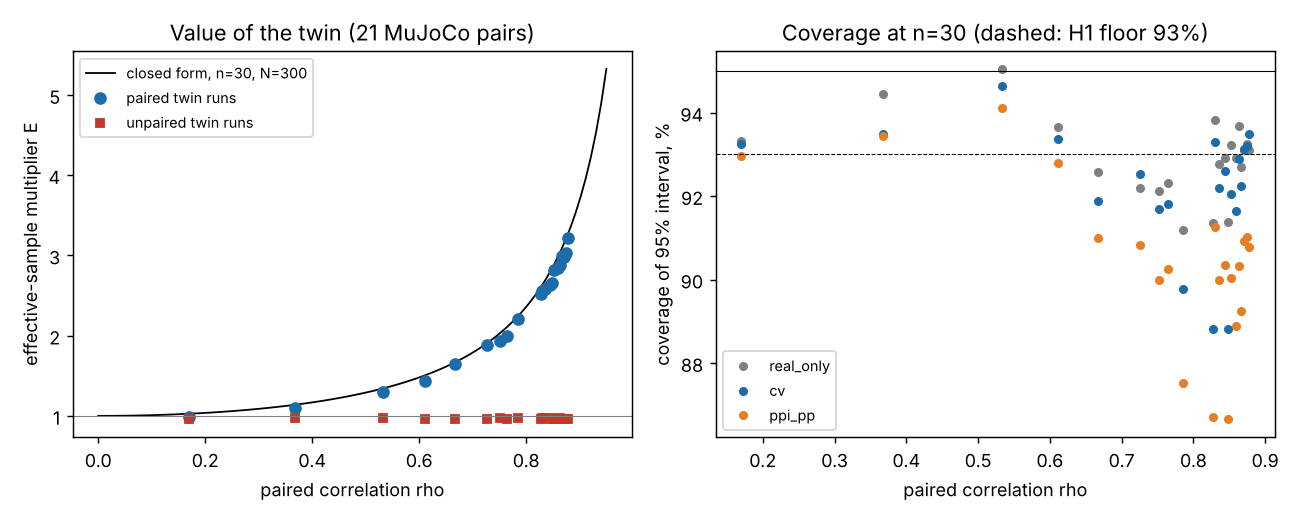
\includegraphics[width=.9\linewidth]{../experiments/m3_benchmark/results/e_vs_rho.png}\caption{Effective-sample multiplier against paired correlation (left) and 95\% interval coverage at $n=30$ (right).}\label{fig:e}\end{figure}
\paragraph{Intervals.} Plug-in $t$ intervals fall below 93\% on 15 (control variate) and 20 (PPI++) of 21 pairs at $n=30$ (worst 88.8\%, 86.7\%); real-only reaches 91.2\% at worst because outcomes are bounded and left-skewed (skewness $-2.4$). A studentised bootstrap lifts mean control-variate coverage from 92.0\% to 93.6\% at 14\% greater width; the percentile bootstrap is worse (90.7\%).

\begin{table}[h]\centering\small
\begin{tabular}{@{}llp{7.6cm}@{}}\toprule
Certificate & Valid? & Width against real-only baseline\\\midrule
Empirical Bernstein, fitted $\lambda$ (3c) & 100\% & 2.1--3.1$\times$ wider\\
Hedged-capital betting (3d) & $\ge$99.5\% & 2--3.4$\times$ wider (mean 2.9 at $n=60$)\\
Pilot-checked $|R-T|$ bound (3e) & 100\% & tighter on 0 of 21 pairs; gap 0.193 against 0.060 at $n=240$\\
Failure-rate bound vs Clopper--Pearson (3f) & $\ge$98.6\% & tighter on 0 of 21; gap 0.056 against 0.041 at $n=240$\\
Anytime sequence (5b) & miss $\le$2.5\% & 74 against 50 median trials to decide at gap 0.10\\\bottomrule
\end{tabular}\caption{Distribution-free certificates built with the twin, $\delta=0.05$, 21 pairs.}\label{tab:cert}\end{table}

\paragraph{Certificates (Table~\ref{tab:cert}).} The twin's variance gain is real for point estimates but none of the five constructions turns it into a tighter guarantee. The binding terms are the range ($1+\lambda$ after rescaling, or $2b$ with $b$ the pilot maximum of $|R-T|$, 0.26--0.36 even at $\rho\approx0.87$) and the price of checking an assumption on a pilot ($\gamma=1-0.01^{1/k}$, 0.056 at $n=240$).

\paragraph{A floor.} \textbf{Theorem.} Let $L$ be any lower confidence bound for $\mu$ with $P(L\le\mu)\ge1-\delta$ for every joint law of $(R,T)$ on $[0,1]^2$, using $m$ paired runs and any number of twin-only runs. With $\epsilon^*=1-(2\delta)^{1/m}$ there is a law with a perfect twin ($R=T=1$) under which $P(L\le 1-\epsilon^*)\ge 1/2$. \emph{Proof.} Under $P_1$, $T=1$ and $R=0$ with probability $\epsilon$ independently ($\mu=1-\epsilon$); under $P_0$, $R=T=1$. Twin-only runs have the same law under both; the paired data coincide with probability $(1-\epsilon)^m$. Validity under $P_1$ gives $\delta\ge P_1(L>1-\epsilon)\ge(1-\epsilon)^mP_0(L>1-\epsilon)$; at $\epsilon^*$, $(1-\epsilon^*)^m=2\delta$, so $P_0(L>1-\epsilon^*)\le1/2$. \hfill$\square$

So a twin cannot reduce the $\approx\ln(1/2\delta)/m$ term, even a perfect one. The floor is 0.0095 at $m=240$, against 0.060 for real-only empirical Bernstein and 0.193 for our bounded-discrepancy bound; on the all-ones sample the exact valid bound is $\delta^{1/m}$, so the floor is tight to about $1.3\times$. There is room for a better construction, but not for one that beats the $\sqrt{\mathrm{var}/m}$ term by more than the twin's variance share. An instance-wise bound involving $\rho$ is open.

\paragraph{A second task (m7a).} To test whether the above is a property of paired inference or of the pendulum, we repeat the benchmark on a MuJoCo cart-pole balanced from a random start by a linear feedback law (unstable plant; a fall ends the episode; outcome is survived fraction times $1-\mathrm{RMS}$ angle$/0.25$), with the same five omitted effects at four swept magnitudes, 21 pairs ($\rho$ 0.37 to 0.86) and 4{,}000 contexts each. The push-noise level was set from a 200-context probe that looked only at $\rho$. The pairing gain replicates: all 16 pairs with $\rho\ge0.75$ have a paired-over-unpaired variance-ratio lower bound of at least 2, and unpaired $E$ is 0.958 to 0.983 everywhere. The predictor result replicates with a clearer margin: Spearman$(E,\rho)=0.909$ against $-0.708$ for the KS distance, difference of absolute values in $[0.021,0.494]$ (pendulum: $[0.008,0.146]$); the rank correlation is below the 0.95 we pre-registered. The interval shortfall does \emph{not} replicate: the control variate or PPI++ falls below 93\% at $n=30$ on 3 of 21 pairs (worst 91.98\%), against 15 and 20 of 21 on the pendulum. The undercoverage is therefore partly task dependent, tied to that outcome's skew, and concentrated on low-$\rho$ pairs where $\lambda$ is noisiest.

\paragraph{An unbounded outcome (m7c).} Re-running the same 21 cart-pole pairs with the tracking cost $\int(100\theta^2+(x-x_{\mathrm{ref}})^2)\,dt$ (no early stop, no upper bound; skewness 1.89) leaves the pairing gain intact (all 17 pairs with $\rho\ge0.75$ have a variance-ratio lower bound of at least 2; unpaired $E$ 0.948 to 0.971). The control variate covers at least 93.3\% at $n=30$ on every pair, while PPI++ falls below 93\% on 18 of 21 (worst 90.2\%), so the interval shortfall is the fixed-weight estimator's, not pairing's. The predictor claim does not survive: Spearman$(E,\rho)=0.884$ against $-0.809$ for KS, difference of absolute values in $[-0.070,0.299]$, which includes 0. We therefore state $\rho$ as a predictor only for bounded outcomes. A certificate for this outcome is available only for the clipped mean $E[\min(R,c)]\le E[R]$ with $c$ the twin's 99.9th percentile: the real-only empirical-Bernstein gap is 27\% of the mean at $n=240$ (median over pairs), but on the three large-friction pairs the twin quantile is below the real outcome and the clipped mean is 14\% to 84\% short.

\paragraph{A twin-chosen range for the unbounded cost (m7d, m7e).} At $q=0.999$ the twin's quantile gives $c=2.009$ for all 21 pools, and clipping loses under 5\% of $E[R]$ on 18 of 21 pairs (median 0.23\%); at $q=0.99$ more than 3\% of real outcomes exceed $c$ on 7 of 21 pairs, so a twin quantile transfers only when the omitted effect is small. The median relative gap of the real-only lower bound on $E[\min(R,c)]$ is 1.51, 0.83, 0.47 and 0.27 at $n=30,60,120,240$. Adding the twin as a control variate on the clipped cost, with the twin mean treated as exactly known (the most favourable case), gives a smaller mean gap than real-only on 0 of 21 pairs at every $n$ (median 0.333 against 0.271 at $n=240$), even where the clipped $\rho$ is near 0.94: doubling the residual range costs more than the smaller residual variance saves. Coverage is 100\% on every cell. The certification result therefore holds on a bounded score, a binary failure indicator and a clipped unbounded cost.

\paragraph{Active selection (H4).} Sampling real contexts in proportion to a gradient-boosting prediction of $|R-T|$ (an $n/3$ uniform pilot fits it), with inverse-probability weights, cuts MSE against uniform at $n=120$ by 17--35\% on the three pairs where twin error is predictable from context (cross-fitted $R^2>0.45$), is 8\% worse in the median on weakly predictable pairs, and loses on 18--19 of 21 pairs at $n=30$--60. Coverage of the plug-in interval is 92.4\% at worst.

\paragraph{Real data (SIMPLER).} We transcribed the published Visual Matching real and SAPIEN success rates \cite{li2024simpler} (36 cells; the eggplant column implies $n=30$, not the 24 in Appendix B, which a transcription test enforces). Raw simulated error has debiased MSE 0.0212 [0.0134, 0.0297], five times the real-only variance at the paper's $n$ (0.0042). A leave-one-cell-out calibrated twin has RMSE 0.118 [0.074, 0.158]; break-even is $n^*=10.1$ real trials [5.1, 26.5]. Pearson $r=0.90$ [0.84, 0.95] between simulated and real rates, so rank agreement is excellent while the level error equals one real-trial standard error at $n\approx15$. Only policy-level rates are published, so the paired control variate is untested on real data. Intervals are bootstrap over cells and optimistic (cells cluster).

\section{Related work}
Prediction-powered inference \cite{angelopoulos2023ppi,angelopoulos2023ppipp}, active inference \cite{zrnic2024active}, design-based surrogates \cite{egami2023surrogates} and multifidelity Monte Carlo \cite{peherstorfer2018survey} supply the estimators; we add context pairing for simulators and measure it. Confidence sequences and betting intervals \cite{howard2021confseq,waudbysmith2020betting} supply the anytime constructions. SIMPLER \cite{li2024simpler} uses simulation as a proxy; \cite{kressgazit2024empirical} sets reporting standards. Rare-event simulation and validation \cite{okelly2018rare,corso2021survey} estimate simulator-side quantities. Sim-to-real work \cite{tobin2017dr,zhao2020survey} closes the gap for training, not for evaluation.

\section{Limitations}
Model-versus-model pairs on two simulated tasks and two outcome forms (a bounded score and an unbounded cost, the latter certified only through a clipped mean); no real-robot episode pairs (the per-episode SIMPLER logs were not obtained); pools are finite populations sampled with and without replacement; one betting construction and one $\delta$ split; certificate comparisons stop at $n=240$; the floor is a worst-case statement and says nothing about instance-wise bounds. Two pre-registered clauses were mis-specified and are corrected in the log (the $\rho\ge0.98$ tier in 3f was empty; the count of pairs with $\rho\ge0.8$ in 5b was 12, not 7).

\section{Conclusion}
A context-paired twin is a variance-reduction device worth up to $1/(1-\rho^2)$ real trials when $\rho$ is high, and about ten real trials at SIMPLER's level of fidelity. It does not shorten a distribution-free certificate at the sample sizes tested, and a worst-case floor shows part of this is unavoidable. Open: an instance-wise bound under a checkable discrepancy assumption; per-episode real pairs; certificates for unbounded outcomes (only a clipped-mean lower bound with a twin-chosen range was tested, m7d, and the twin did not shorten it, m7e; the twin mean was taken as known).

\paragraph{Reproducibility.} \texttt{reproduce.sh} lists one command per figure and table; code, data and the pre-registration log are in the repository under MIT licence. AI assistance (Claude Code) wrote the code and this draft; it implies no affiliation with or endorsement by any cited author.
\bibliographystyle{plain}
\bibliography{refs}
\end{document}
